%! Author = Frederik Bußmann
%! Date = 22.06.2023

\section{Umsetzung der CI-Strategie} \label{sec:04-implementation}

% @TODO: Einleitung überarbeiten

Im Folgenden wird die zuvor konzipierte\ \acrshort{ci}-Strategie in die Praxis umgesetzt und dabei in einer Fallstudie
exemplarisch auf ein Projekt angewandt.
Zunächst wird das ausgewählte Projekt vorgestellt, um einen Kontext für die anschließende Implementierung zu schaffen.
Dabei werden die spezifischen Anforderungen und Besonderheiten des Projekts hervorgehoben.
Im Anschluss daran wird die praktische Umsetzung der \acrshort{ci}-Strategie beschrieben, wobei sowohl die technischen
Aspekte als auch die organisatorischen Prozesse berücksichtigt werden.

\subsection{Projekthintergrund} \label{subsec:04-implementation-1}

% @TODO: Text verbessern

Bei dem Shopware-Projekt, in welchem die\ \acrshort{ci}-Strategie implementiert werden soll, handelt es sich um einen
Anbieter von Kochutensilien.
Der Shop soll dabei auf der Basis von Shopware 6 neu entwickelt werden und das zuvor erstellte Konzept in der Praxis
einsetzen.
Ziel ist es, durch die Integration der untersuchten \acrshort{ci}-Praktiken eine robuste, skalierbare und effiziente
Entwicklungsumgebung zu schaffen, die den Anforderungen moderner Online-Shops gerecht wird.
Dabei wird das zuvor ausgearbeitete \acrshort{ci}-Konzept als Leitfaden für die Entwicklung und Optimierung des Shops
herangezogen.
Hierzu wird zunächst eine Shopware-Instanz aufgesetzt, welche anschließend über den Standardumfang der Software um ein
eigenes Theme und einige Plugins zur Anpassung verschiedener Bereiche des Shops ergänzt wird.
Die für den Shop angedachten Eigenentwicklungen umfassen folgende Plugins:

\begin{itemize}
    \item {
        \textbf{Eigene Produktkacheln auf Listing-Seiten}\par
        Bei Varianten-Artikeln wird keine direkte Auswahlmöglichkeit angeboten, stattdessen werden individuell
        gestaltete Produktkacheln präsentiert.
    }

    \item {
        \textbf{Eigener Produkt-Typ\ \glqq Rezept\grqq}\par
        Dieser spezielle Produkttyp kann vom Kunden betrachtet, aber nicht gekauft werden.
        Er dient zur Präsentation von Rezepten, die mit den im Shop erhältlichen Produkten zubereitet werden können.
    }
\end{itemize}

Einige weitere benötigte Features des Shops, wie eine Filialsuche und Social-Media-Feeds werden dabei über
Drittanbieter-Plugins gelöst, um Entwicklungszeit einzusparen.

\subsection{Implementierung des Konzepts} \label{subsec:04-implementation-2}

Nachfolgend wird das als Fallstudie vorgesehene Shopware-Projekt anhand der untersuchten\ \acrshort{ci}-Praktiken
implementiert.
Zunächst wird gemäß des Konzepts eine Analyse der zur Verfügung stehenden\ \acrshort{ci}-Tools durchgeführt,
woraufhin Technologien für die Nutzung innerhalb des Projekts ausgewählt werden.
Anschließend wird die Projekt-Umgebung für die Nutzung von\ \acrshort{ci} aufgesetzt und das Shopware-Projekt
installiert und vorbereitet.
Daraufhin wird die Pipeline für das erstellte Projekt angelegt.
Hierbei werden die Phasen und Jobs angelegt und\ \acrshort{ci}-Tools konfiguriert, um automatisierte Tests und Analysen
durchführen zu können.
Nachdem das Projekt initialisiert wurde und die Pipeline funktionsfähig ist, wird die Implementierung der eigentlichen
Shop-Funktionen erläutert, wobei der Fokus auf die kontinuierliche Prüfung der Features durch die Pipeline gerichtet
ist.

\subsubsection{Auswahl von\ \acrshort{ci}-Tools}

% @TODO: Text verlängern, verbessern

Bevor mit der Implementierung des Projekts begonnen werden konnte, musste zunächst analysiert werden, welche Tools
innerhalb des Projekts eingesetzt werden können.
Hierfür wurde eine Analyse der vorhandenen\ \acrshort{ci}-Tools durchgeführt, anhand dessen eine Auswahl an für das
Projekt zu nutzenden Technologien getroffen wurde:\\

\hspace{0.025\textwidth}%
\begin{minipage}{0.5\textwidth}
    \textbf{Version Control System}
    \vspace{-2mm}
    \begin{itemize}
        \setlength\itemsep{0em}
        \item GitLab
        \item[]
    \end{itemize}
\end{minipage}%
\begin{minipage}{0.475\textwidth}
    \textbf{Pipeline-Runner}
    \vspace{-2mm}
    \begin{itemize}
        \setlength\itemsep{0em}
        \item GitLab CI/CD
        \item[]
    \end{itemize}
\end{minipage}

\hspace{0.025\textwidth}%
\begin{minipage}{0.5\textwidth}
    \textbf{PHP Testing Tools}
    \vspace{-2mm}
    \begin{itemize}
        \setlength\itemsep{0em}
        \item PHPUnit
        \item Infection
        \item[]
    \end{itemize}
\end{minipage}
\begin{minipage}{0.475\textwidth}
    \textbf{JavaScript Testing Tools}
    \vspace{-2mm}
    \begin{itemize}
        \setlength\itemsep{0em}
        \item Jest
        \item Cypress
        \item[]
    \end{itemize}
\end{minipage}

\hspace{0.025\textwidth}%
\begin{minipage}{0.5\textwidth}
    \textbf{PHP Static-Code-Analysis Tools}
    \vspace{-2mm}
    \begin{itemize}
        \setlength\itemsep{0em}
        \item PHP\_CodeSniffer
        \item PHP Mess Detector
        \item PHPStan
        \item Deptrac
        \item License Checker
        \item Security Checker
        \item[]
    \end{itemize}
\end{minipage}
\begin{minipage}{0.475\textwidth}
    \textbf{JavaScript Static-Code-Analysis Tools}
    \vspace{-2mm}
    \begin{itemize}
        \setlength\itemsep{0em}
        \item Eslint
        \item Danger JS
        \item License Checker
        \item AuditJS
        \item[]
        \item[]
        \item[]
    \end{itemize}
\end{minipage}

Eine vollständige Übersicht und Beschreibung der einzelnen Tools kann aus Anhang\ \ref{sec:appendix-1} entnommen werden.

\subsubsection{Aufsetzen der Projekt-Umgebung}

% Aufsetzen der Docker-Umgebung, Installieren von Shopware, VCS check-in, Aufsetzen Dev-, Staging- und Production-Server

Nach dem Festlegen der zu verwendenden Technologien wurde mit der Implementierung des Projekts begonnen, wobei
zuerst eine Umgebung für die Ausführung von Shopware und der gewählten\ \acrshort{ci}-Tools erstellt wurde.
Hierbei wurde sich für die Nutzung von Docker als Containerization-Technologie entschieden, da Shopware selbst ein
Docker-Image für das Betreiben der Plattform bereitstellt.\footpartcite{shopware-docker}
Auf der Basis des bereitgestellten Images wurde eine Shopware-Instanz aufgesetzt und anschließend eine Datenbank
angebunden.
Diese wurde, um in der\ \acrshort{ci}-Pipeline wiederverwendet werden zu können, auch aus einem Docker-Image
instanziiert.
Nach der Shopware-Installation wurden Grundkonfigurationen vorgenommen und erste manuelle Tests durchgeführt, um
sicherzustellen, dass die Instanz funktional ist.
\\\\ % @TODO: Branching-Strategie erklären
Nachdem die lokale Entwicklungsumgebung erstellt wurde, konnte mit der Vorbereitung für die Umgebung der Pipelines
begonnen werden.
Hierzu wurde das gesamte Projekt in GitLab hinterlegt und ein Branching-Modell eingeführt, um sicherzustellen, dass
neue Features und Bugfixes vor der Integration in den Hauptzweig (\shellinline{main}) in isolierten Branches entwickelt
werden.
Neben dem\ \shellinline{main}-Branch, welcher als Deployment-Ziel die Produktionsumgebung hinterlegt hat, wurden auch
ein Development-Branch (\shellinline{development}) und -Server angelegt und eine Staging-Umgebung aufgesetzt.
Der Staging-Server ist dabei ein variables Deployment-Ziel, für welches die Auslieferung von
\shellinline{release}-Branches vorgesehen ist.
Die hierbei verwendete Branching-Strategie nennt sich\ \glqq Git-Flow\grqq.\footpartcite{git-flow}

\subsubsection{Erstellen der Pipeline}

% Anlegen der Pipeline inklusive automatisierter Tests, Static-Analysis, Monitoring, etc.

Zunächst soll eine grundlegende Pipeline definiert werden, die bei jeder Integration in einen Branch, ungeachtet der
definierten Deployment-Umgebung läuft.
Diese Pipeline durchläuft eine Build- und eine Testing-Stage.
Im Build-Prozess werden die \acrshort{ci}-Tools und die Abhängigkeiten der Shopware-Platform installiert.
Der Testing-Prozess umfasst zunächst alle für die Strategie ausgewählten Test- und \acrshort{qa}-Tools, inklusive
lang-andauernder Tests durch End-to-End-Testing.
Im späteren Verlauf der Entwicklung besteht durch Gitlab CI/CD die Möglichkeit, diese Tests nur in Branches mit
definierter Deployment-Umgebung durchführen zu lassen, falls dessen Laufzeit zu groß wird ($> 10min$).

\begin{figure}[H]
    \centering
    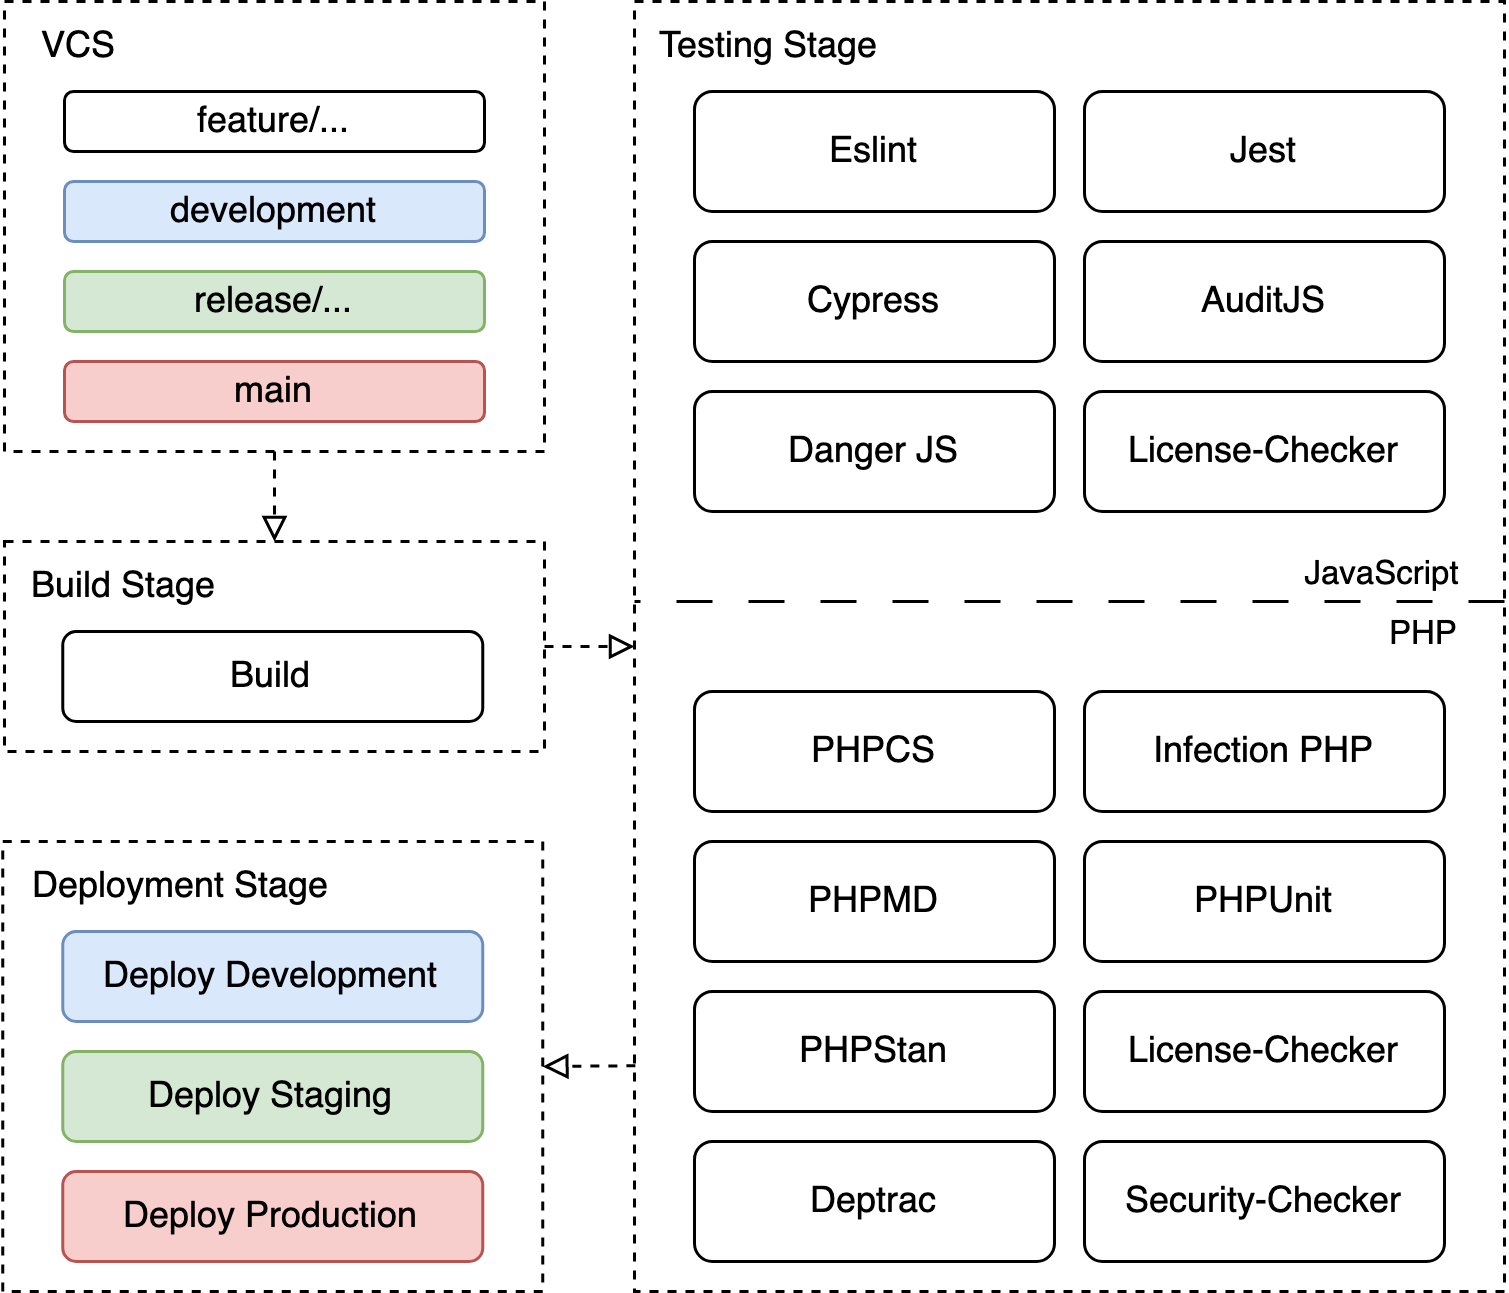
\includegraphics[width=0.7\textwidth]{images/content/ci-pipeline-concept}
    \captioncite[Eigene Darstellung]{}{Visualisierung der implementierten\ \acrshort{ci}-Pipeline}
    \label{fig:ci-pipeline-concept}
\end{figure}

\subsubsection{Implementierung der Shop-Funktionen}

% Implementierung der individuellen geplanten Funktionen des Shops anhand der Kunden-Anforderungen
% Fokus auf Nutzung der CI-Pipeline und der Docker-Umgebung und sowas alles

\clearpage
